%955
\newpage
\section{プログラムと\ruby{画像}{が|ぞう}ファイルについて知ろう}


\subsection{絵を出してみよう}


ゲームを作る場合には、きれいな絵を出したいですよね。

ここでは、HSPで文字だけでなく、絵を出す方法について学んでいきましょう。

\bigskip

まずは、簡単なプログラムから見てみましょう。

スクリプトエディタの、ファイル→「開く」メニューから「celput.hsp」を読み込んでください。

終わったら、さっそく[F5]キーを押してプログラムを実行してみましょう。


\begin{figure}[H]
    \begin{center}
      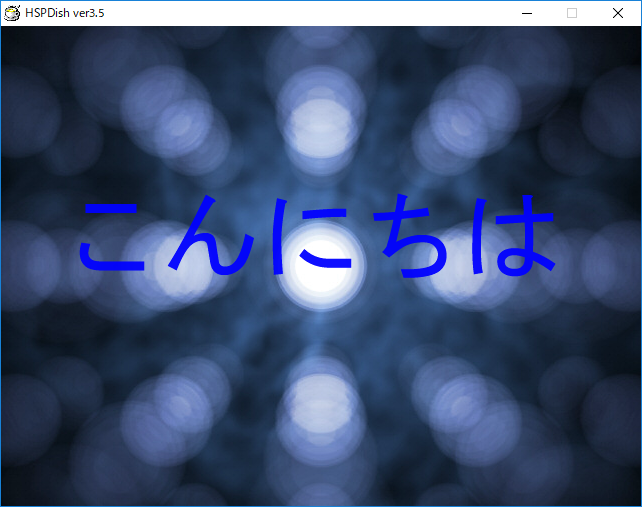
\includegraphics[keepaspectratio,width=10.028cm,height=7.909cm]{text04-img/s_celput.png}
      \caption{celput.hspの実行画面}
    \end{center}
    \label{fig:prog_menu}
\end{figure}


今度は、\ruby{背景}{はい|けい}に絵が出ました。

この絵は、あらかじめ「sozai1.jpg」というファイルで\ruby{用意}{よう|い}されているものです。

実際に絵を出すためには、画像ファイルと呼ばれる絵のデータが必要になります。

それが、「sozai1.jpg」になります。(画像ファイルは、GIMPツールや、ブラウザなどで開くことができます。)


絵を出すためには、2つの命令を使う必要があります。1つ目のcelloadは、必要な絵の素材を知らせるための命令です。これにより、指定された素材を表示する準備をします。

\begin{description}
    \item \textgt{\bf \ \ celload “画像ファイル名” , 絵の番号\ \ \ \ \texttt{← 絵を出す準備をする}}
\end{description}


一度、celload命令によって\ruby{登録}{とう|ろく}された絵は、celput命令によって表示させることができます。

celload命令は、最初の1回だけ実行すれば良いです。以降は、celput命令によって、mes命令やboxf命令と同じように絵を出すことができるようになります。


celput命令は、以下のように書くことができます。




\begin{description}
    \item \textgt{\bf celput 絵の番号}
\end{description}



絵の番号というのは、celload命令で指定していた番号のことです。

出すための絵を登録する時に、1,2,3,4…というように、別々な番号を\ruby{割}{わ}り\ruby{振}{ふ}っておいて、同時に色々な絵を出せるようにするための仕組みです。

最初は、番号1を使っておきましょう。


\begin{figure}[H]
    \begin{center}
      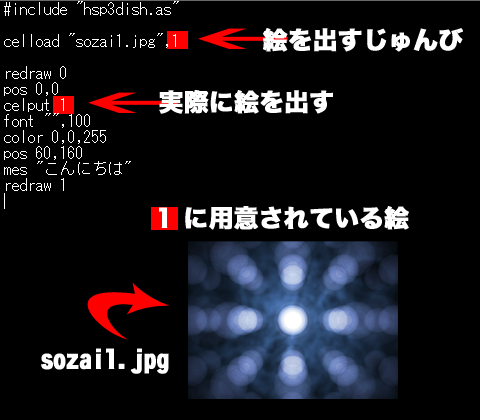
\includegraphics[keepaspectratio,width=12.806cm,height=11.206cm]{text04-img/s_celload.png}
    \end{center}
    \label{fig:prog_menu}
\end{figure}


つまり、


\begin{description}
    \item \textgt{\bf \ \ celload “sozai1.jpg”,1}
\end{description}

は、番号1で「sozai1.jpg」の絵を表示するための準備をするという意味になります。

celputで指定した番号に準備された絵を表示します。

表示する位置は、mes命令などと同じようにpos命令で指定された位置になります。

準備する画像のファイルは、プログラム(.hsp)がある場所と同じフォルダに入れておく必要があります。

画像ファイル、「sozai1.jpg」は、04フォルダ内にあるはずです。


celload命令とcelput命令、絵を出す番号と画像ファイルの\ruby{関係}{かん|けい}をよく覚えておきましょう。

\newpage
\subsection{例題に挑戦しよう}


終わってしまった人は、以下の例題にも挑戦してみよう。


・色々な絵と文字を表示しよう

・自分で用意した絵を表示する

例題の考え方がわからない時は、近くのTAか先生に聞いてください。

わからない所は、そのままにせず、必ず答えを見つけてから先に進みましょう。

%1095
\newpage
\subsection{例題4-4 色々な絵と文字を表示する}


\begin{description}
    \item \textgt{\bf 考え方}
\end{description}

絵と文字を表示するプログラム(celput.hsp)を改造してみましょう。

\begin{description}
    \item \textgt{\bf \ \ celload “sozai1.jpg”,1}
\end{description}


は「sozai1.jpg」という画像ファイルを表示するための準備をします。

[資料] 背景として使える画面の一例

   ( sozai1.jpg 〜 sozai20.jpg )


\begin{figure}[H]
    \begin{center}
      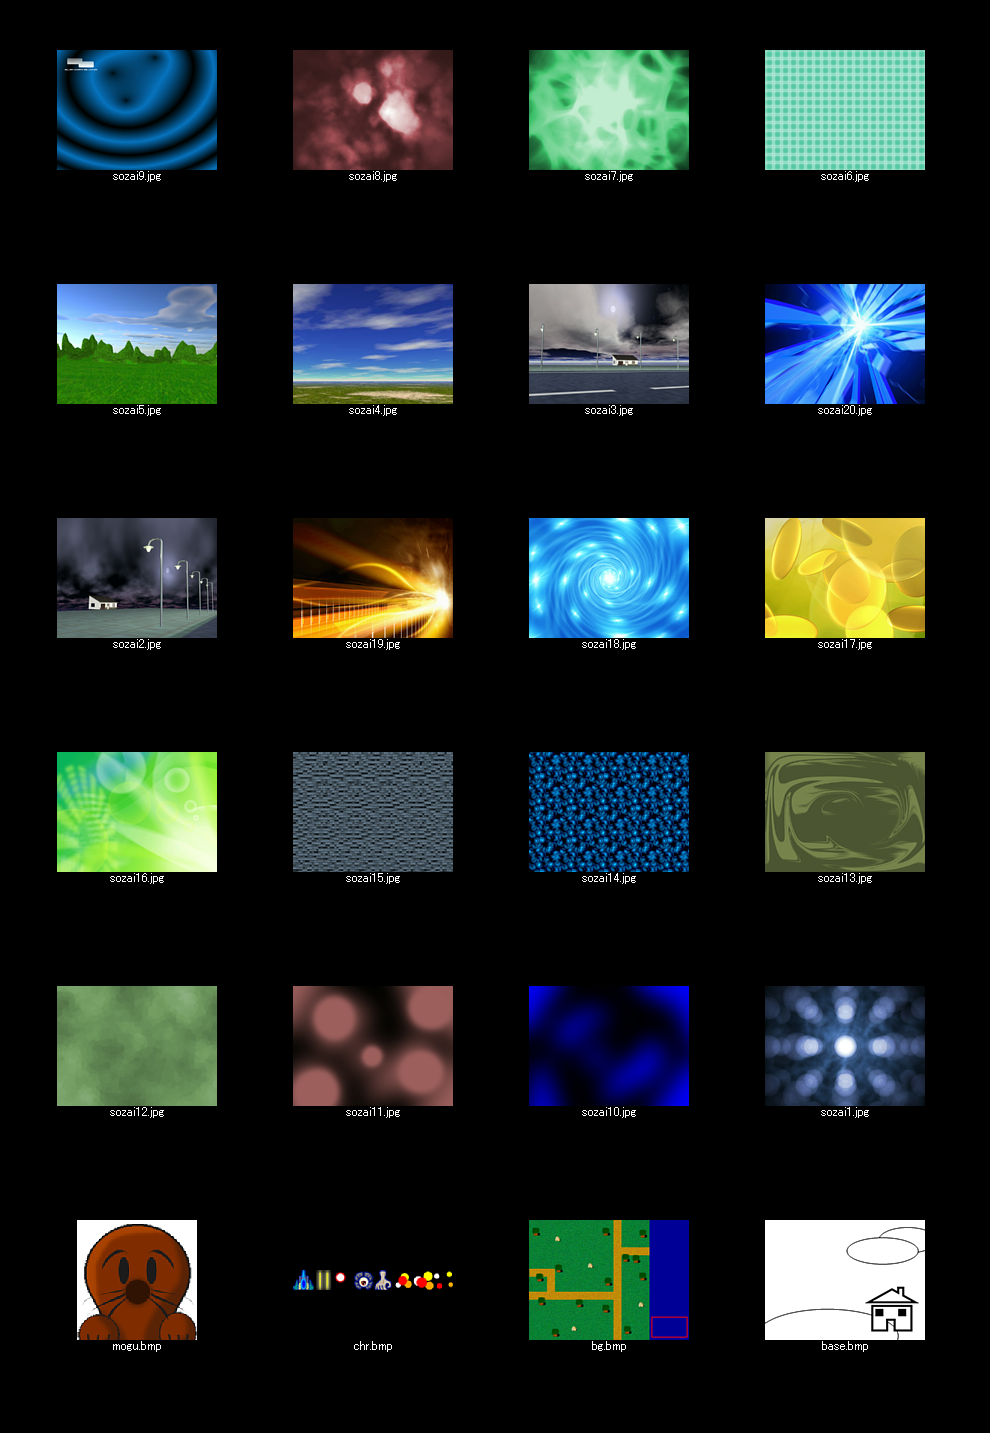
\includegraphics[keepaspectratio,width=14.843cm,height=17.609cm]{text04-img/s_sozai.png}
    \end{center}
    \label{fig:prog_menu}
\end{figure}

試しに、celload命令で指定している画像ファイル名を他のものに変更して、実行してみましょう。

このように自由な絵を使って画面を作っていくことができます。


\begin{description}
    \item \textgt{\bf 例題4-4 答え}
\end{description}



「04」フォルダには、自由に使える\ruby{素材}{そ|ざい}として「sozai1.jpg」から「sozai20.jpg」まで20種類の画像ファイルが含まれています。

[F5]キーを押して改造した画面がきちんと表示されるかどうか確認しましょう。

mes命令、font命令、color命令、pos命令も書き換えることで、違ったメッセージを表示させることができます。

改造ができたらTAや周りの友達にも見せてあげましょう。

%1158

%8/31
%1158
\newpage
\subsection{例題4-5 自分で用意した絵を表示する}

\begin{description}
    \item \textgt{\bf \ \ 考え方}
\end{description}


絵と文字を表示するプログラム(celput.hsp)を改造して自分で用意した絵を出してみましょう。

準備する画像のファイルは、プログラム(.hsp)がある場所と同じフォルダに入れておく必要があります。

\ \ celput.hsp

\ \ sozai1.jpg

が同じディレクトリにあることを確認しましょう。

同じように「04」フォルダの中に、皆さんが自分で画像を作ったり、コピーして使用することもできます。

\begin{description}
    \item \textgt{\bf \ \ 例題4-5 答え}
\end{description}


[F5]キーを押して正しい画像が表示されるかどうか確認しましょう。

改造ができたらTAや周りの友達にも見せてあげましょう。

プログラムをあまり改造しすぎると、動かなくなったり、パソコンの動きが遅くなってしまうことがあります。その時は、先生に聞くか、元のファイル(celput.hsp)をもう一度コピーして使ってみてください。

%1218

%1218
\newpage
\subsection{絵を\ruby{重}{かさ}ねて表示してみよう}


もう少し別な絵を表示してみましょう。

スクリプトエディタの、ファイル→「開く」メニューから「apple.hsp」を読み込んで実行してみてください。

\begin{figure}[H]
    \begin{center}
      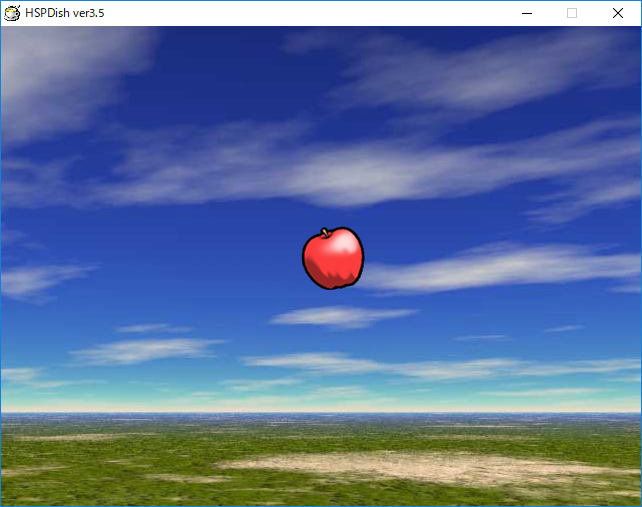
\includegraphics[keepaspectratio,width=9.634cm,height=7.599cm]{text04-img/s_applehsp.png}
      \caption{apple.hspの実行画面}
    \end{center}
    \label{fig:prog_menu}
\end{figure}

今度は、画面の中央に「りんご」が表示されていることに気付いたでしょうか。


実は、このプログラムでは背景と「りんご」の2つの画像を使っています。

背景の上に「りんご」を表示しているのです。


\begin{figure}[H]
    \begin{center}
      
\includegraphics[keepaspectratio,width=2.249cm,height=2.249cm]{text04-img/s_apple.png}
      \caption{リンゴの画像( apple.png )}
    \end{center}
    \label{fig:prog_menu}
\end{figure}


\begin{figure}[H]
    \begin{center}
      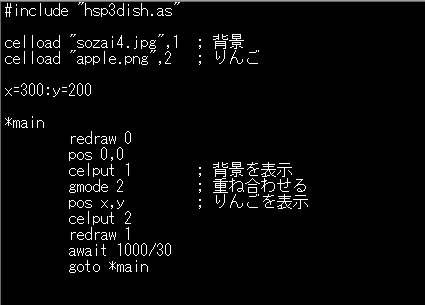
\includegraphics[keepaspectratio,width=11.245cm,height=8.07cm]{text04-img/s_applehspsrc.png}
    \end{center}
    \label{fig:prog_menu}
\end{figure}

このように複数の番号を登録して、celput命令を使うことで絵を重ねて表示することができます。

そのために、gmodeという新しい命令が使われています。


\begin{description}
    \item \textgt{\bf \ \ (HSPのルール)}
\end{description}


\begin{description}
    \item \textgt{\bf \ \ 画像を重ねる設定をするにはgmode命令を使います}
    \item \textgt{\bf \ \ gmodeの後、スペースに続けてコピーモードを示す数字を指定します}
    \item \textgt{\bf \ \ コピーモードは、以下のような意味があります}
    \item \textgt{\bf \ \ \ \ 0のとき \ \ \ \ \ \ \ : 画像のまま表示}
    \item \textgt{\bf \ \ \ \ 1か2のとき \ \ \ : 透明な部分は背景を残して表示}
    \item \textgt{\bf \ \ \ \ 3のとき \ \ \ \ \ \ \ : 透明度を変えて表示}
\end{description}

「gmode 2」を指定することで、リンゴの透明な部分は背景が表示されて、きれいに重なっているように見えています。試しに、「gmode 0」にしてリンゴの絵がどのように表示されるか確認してみましょう。

リンゴのように透明な部分がある絵は、以前にも使ったGIMPツールで作ったり、確認することができます。GIMPは、画像ファイルの右クリックメニューから「GNU Image Manipulation Program」を選択することで起動させることができます。

\begin{figure}[H]
    \begin{center}
      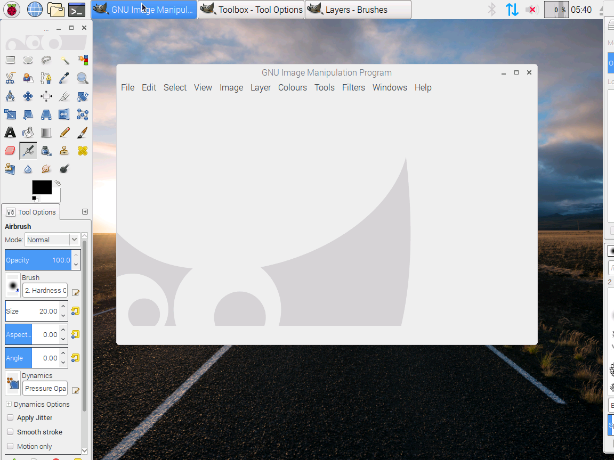
\includegraphics[keepaspectratio,width=7.091cm,height=5.318cm]{text04-img/s_gimpboot.png}
      \caption{GIMPを起動した画面}
    \end{center}
    \label{fig:prog_menu}
\end{figure}

celput命令には、実はもっと多くのパラメーターがあります。



\begin{description}
    \item \textgt{\bf \ \ celput 絵の番号, \ruby{分割画像}{ぶん|かつ|が|ぞう}No. , \ruby{横方向}{よこ|ほう|こう}の\ruby{表示倍率}{ひょう|じ|ばい|りつ}, \ruby{縦方向}{たて|ほう|こう}の\ruby{表示倍率}{ひょう|じ|ばい|りつ}, \ruby{回転角度}{かい|てん|かく|ど}}
\end{description}



\begin{description}
    \item \textgt{\bf \ \ 横方向の表示倍率=0.0〜    : 横方向の表示倍率(\ruby{実数}{じっ|すう})}
    \item \textgt{\bf \ \ 縦方向の表示倍率=0.0〜    : 縦方向の表示倍率(\ruby{実数}{じっ|すう})}
    \item \textgt{\bf \ \ 回転角度=0.0〜6.28…(2π) : 回転角度(\ruby{実数}{じっ|すう})}
\end{description}

絵を自由な大きさ(\ruby{倍率}{ばい|りつ})、\ruby{角度}{かく|ど}で出すことができるようになっています。

通常は、倍率1、角度0の状態で表示されます。

分割画像No.は、1つの画像を複数の小さなブロックに分けて表示するための機能です。

(これについては、また別の機会に説明します。)

試しに、表示倍率や角度を変えてみて、どのように表示が変わるか確認してみましょう。

また、余裕がある人は、文字を重ねてさらに複雑な画面を作ることに挑戦してください。


%1372

%1372
\newpage
\subsection{絵を動かしてみよう}



今度は、表示した絵を動かしてみることにしましょう。

絵が動くことで、ゲームやアニメーションなどさらに\ruby{応用}{おう|よう}が広がります。

そのために覚えておかなければならないのが、\ruby{変数}{へん|すう}です。


変数について学んだことを覚えていますか?


\begin{description}
    \item \textgt{\bf \ \ (HSPのルール)}
    \item \textgt{\bf \ \ 「変数の名前=数値」で変数に値を入れることができる(代入)}
    \item \textgt{\bf \ \ 変数に数値を入れておくとパラメーターとして使える}
    \item \textgt{\bf \ \ mes命令の中で「+変数」を書くことで変数の中身を表示できる}
\end{description}

「a=100」と置くと、変数aに100という数字が記憶されます。

これを使って、いままで数字を書いていた部分に変数を代わりに書いて数字を変化させることができます。

スクリプトエディタの、ファイル→「開く」メニューから「fall.hsp」を読み込んで実行してみてください。



\begin{figure}[H]
    \begin{center}
      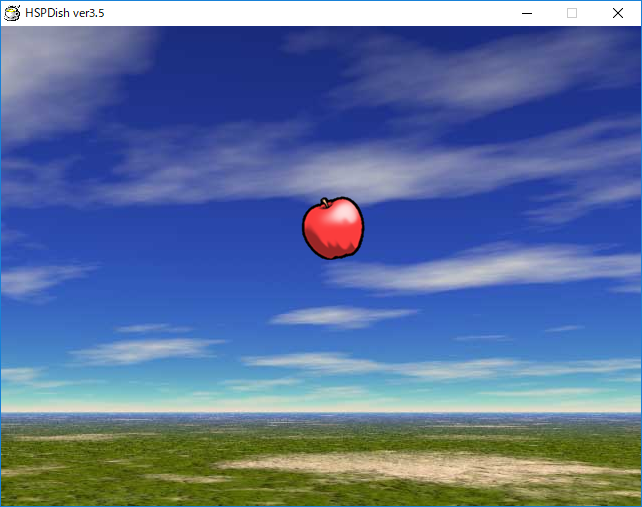
\includegraphics[keepaspectratio,width=9.183cm,height=7.241cm]{text04-img/s_fall.png}
      \caption{fall.hspの実行画面}
    \end{center}
    \label{fig:prog_menu}
\end{figure}

今度はリンゴが動いているのがわかると思います。


\begin{figure}[H]
    \begin{center}
      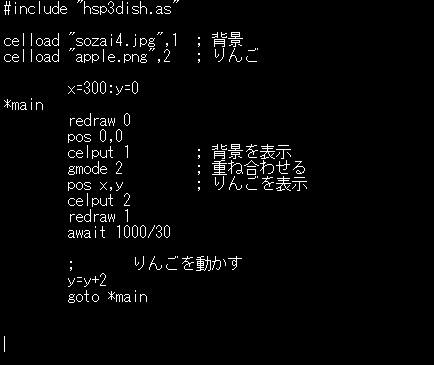
\includegraphics[keepaspectratio,width=10.954cm,height=9.213cm]{text04-img/s_fallsrc.png}
    \end{center}
    \label{fig:prog_menu}
\end{figure}


プログラムを見てみましょう。

変数xと変数yが、リンゴの横、縦の位置を\ruby{記憶}{き|おく}しています。

最初に「x=300:y=0」の行で、変数xに300を、変数yに0を\ruby{代入}{だい|にゅう}しています。



\begin{description}
    \item \textgt{\bf \ \ (HSPのルール)}
    \item \textgt{\bf 「:」の\ruby{記号}{き|ごう}を入れると、行を分けたのと同じように別な命令を書ける}
    \item \textgt{\bf \ \ 「:」の記号を使って1行にたくさんの命令を書くことができる}
\end{description}

「pos x,y」がありますので、celputする時の位置を変数x,yで変えられるようになっています。

つまり、横の位置が変数x、縦の位置が変数yに記憶されていることになります。

実際にリンゴの位置を変えているのが、「y=y+2」の部分です。

ここを繰り返し実行することで、変数yの値が2ずつ増えていきます。


\begin{description}
    \item \textgt{\bf \ \ (HSPのルール)}
    \item \textgt{\bf \ \ 「数式とは、数値と変数、またはそれらを計算式でつなげて書くこと}
    \item \textgt{\bf \ \ 「+」は足し算、「-」は引き算、「*」は掛け算(×)、「/」は割り算(÷) }
\end{description}



「y=y+2」は変数yに記憶されている数字に2を足すという意味だと覚えておきましょう。

これで、縦の位置が少しずつ変化するようになります。
\newpage
\subsection{例題に挑戦しよう}


終わってしまった人は、以下の例題にも挑戦してみよう。

・色々な動きに挑戦してみよう

・自分で用意した絵を動かして表示する

例題の考え方がわからない時は、近くのTAか先生に聞いてください。

わからない所は、そのままにせず、必ず答えを見つけてから先に進みましょう。

%1522

%1522
\newpage
\subsection{例題4-6 色々な動きに挑戦してみよう}


\begin{description}
    \item \textgt{\bf \ \ 考え方}
\end{description}

りんごを動かすプログラム(apple.hsp)を改造して動きを変えてみましょう。


\begin{figure}[H]
    \begin{center}
      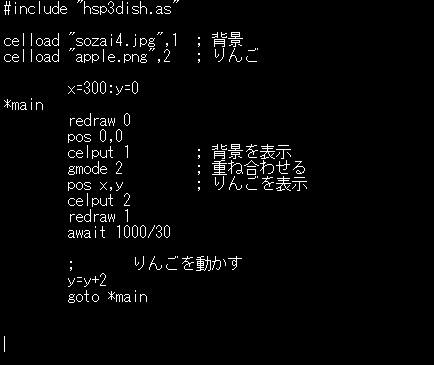
\includegraphics[keepaspectratio,width=10.954cm,height=9.213cm]{text04-img/s_fallsrc.png}
    \end{center}
    \label{fig:prog_menu}
\end{figure}

変数xとyが、横と縦の位置を記憶していることはわかりましたか。

「y=y+2」という計算で下に向かって絵が動いていきます。

もっと速く動かすにはどうすればいいでしょうか?

別な方向、たとえば左から右、下から上に動かす方法を考えてみましょう。


\begin{description}
    \item \textgt{\bf \ \ 例題4-6 答え}
\end{description}



変数xの値を計算で変えることで横方向に、変数yの値を計算で変えることで縦方向に動かすことができます。

たとえば、「x=x+2」は右に、「y=y-2」は上に動くことになります。

計算で使っている「2」という数字は、1つのコマで動く大きさになります。

この値を変えることで、動く速さも変わります。大きな数字で速い速度、小さな数字で遅くなることを確認してみましょう。

%1578

%1578
\newpage
\subsection{例題4-7 自分で用意した絵を動かして表示する}


\begin{description}
    \item \textgt{\bf \ \ 考え方}
\end{description}



apple.hspのプログラムを使って、自分で作った絵を動かすようにしてみましょう。

表示させるための画像は、GIMPツールで作ったり、確認することができます。GIMPは、Raspberry
Piメニューからグラフィックス→「GNU Image Manipulation Program」をクリックすることで起動させることができます。

りんごの画像は、「apple.png」です。

開くメニューから、「apple.png」を読み込んで編集してください。

背景にあたる部分は、\ruby{消}{け}しゴムで消す\ruby{必要}{ひつ|よう}があるので注意してください。


\begin{figure}[H]
    \begin{center}
      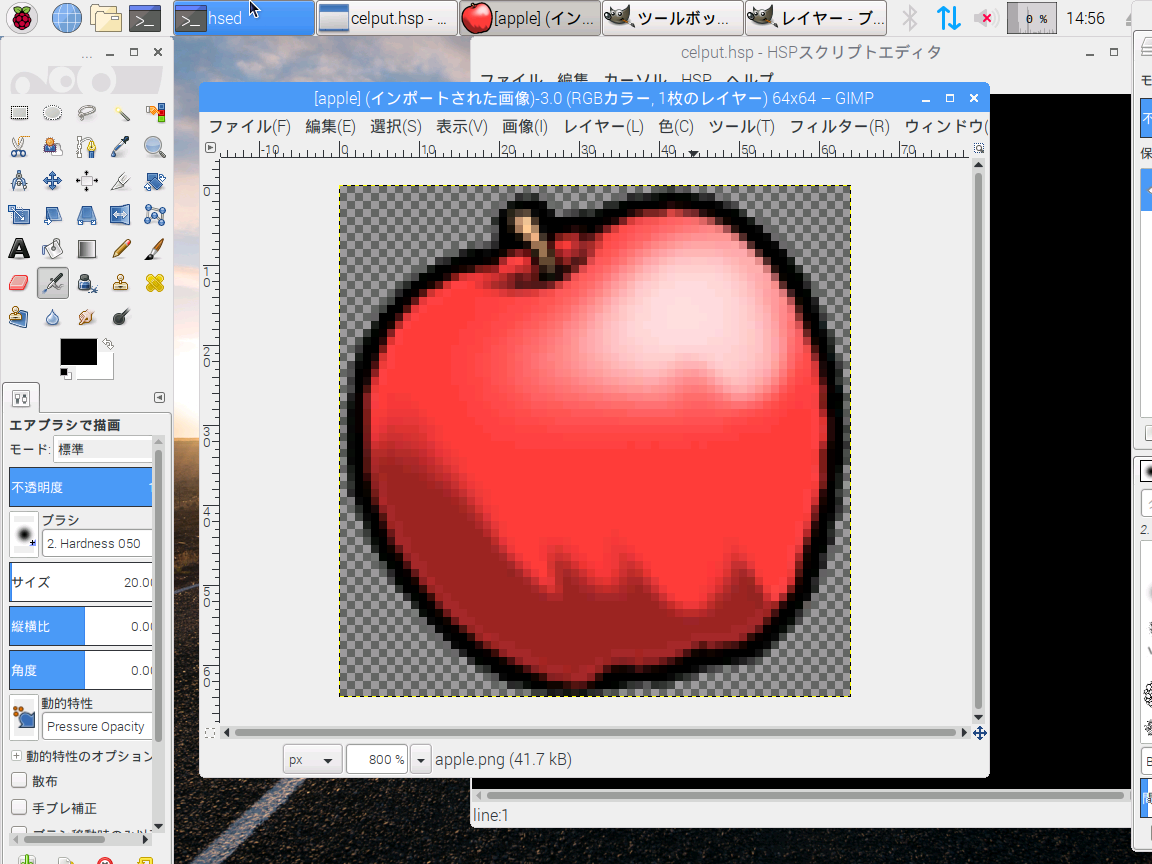
\includegraphics[keepaspectratio,width=11.712cm,height=8.784cm]{text04-img/s_gimpedit.png}
      \caption{GIMPの編集画面}
    \end{center}
    \label{fig:prog_menu}
\end{figure}

% \bfseries  "\ \"
\begin{description}
    \item \textgt{\bf 例題4-7 答え}
\end{description}



GIMPで修正できたら、[F5]キーを押して改造した人がきちんと表示されるかどうか確認しましょう。

自分で別な画像ファイルを用意した場合は、

\begin{description}
    \item \textgt{\bf \ \ celload “apple.png”,2}
\end{description}


のファイル名を修正してください。

もとのりんご画像に戻したい時は、元のファイル(apple.png)をもう一度コピーして使ってみてください。

% Jump Action:

%1644

